\documentclass[10pt]{article}
\usepackage[margin=1in]{geometry}
\usepackage[shortlabels]{enumitem}
%\setcounter{secnumdepth}{0}
\usepackage{amssymb,amsmath,amsthm}
\usepackage{graphicx}
\usepackage{caption}
\usepackage{fancyhdr, lastpage}
\pagestyle{fancy}
\fancyhf{}
\lhead{Daniel Standage}
\chead{GDCB 511, 9:00am MWF}
\rhead{Lecture Notes: 13 Jan, 2012}
%\cfoot{Page \thepage{} of \protect\pageref*{LastPage}}
\usepackage{varioref}
\labelformat{equation}{(#1)}
\usepackage[colorlinks,linkcolor=blue]{hyperref}

\newenvironment{mitemize}
{
  \begin{itemize}
  \setlength{\itemsep}{1pt}
  \setlength{\parskip}{0pt}
  \setlength{\parsep}{0pt}}{\end{itemize}
}

\newenvironment{menumerate}
{
  \begin{enumerate}
  \setlength{\itemsep}{1pt}
  \setlength{\parskip}{0pt}
  \setlength{\parsep}{0pt}}{\end{enumerate}
}


\begin{document}

\section*{Prokaryotic transcription}

\subsection*{Regulatory elements}
\begin{mitemize}
  \item core promoter: -10 box and -35 box
  \item UP element: enhances transcriptional production (as much as 30x)
\end{mitemize}

\subsection*{RNA Polymerase}
\begin{figure}[h] \centering
  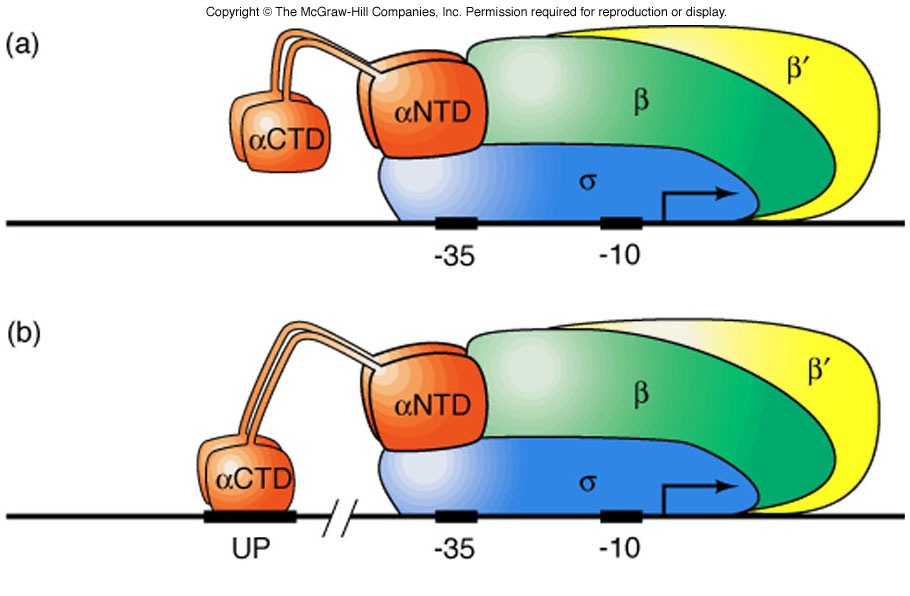
\includegraphics[width=240px]{rna-pol-holoenzyme.jpg}
\end{figure}
\begin{mitemize}
  \item $\sigma$ factor very important to binding; incomplete complex can bind, but complete holoenzyme binds much better
  \item function of $\alpha$ factor proven by 1) mutating UP element and 2) modifying C-terminal domain (CDT)
\end{mitemize}

\subsection*{Transcription termination}
\begin{mitemize}
  \item intrinsic termination: hairpin formation followed by AT-rich region (weak binding)
  \item rho-dependent termination: hairpin formation followed by transcript release by rho helicase
\end{mitemize}

\subsection*{Further reading}
Two papers from the recent literature discuss transcription.
We have been assigned to read them over the long weekend, and we will be tested later on the material.
\begin{mitemize}
  \item \url{http://dx.doi.org/10.1016/j.cell.2011.10.041}
  \item \url{http://dx.doi.org/10.1016/j.cell.2011.11.033}
\end{mitemize}

\end{document}
